\chapter{Resultados} \label{resultado}

Nós inicialmente analisamos erro e discrepância nos 12.502 endereços de São Paulo. Abaixo estão os totais de geocodificações bem-sucedidas para cada API:

\begin{itemize}
    \item TomTom: 11.370 endereços.
    \item Google Maps: 9.389 endereços.
    \item Mapbox: 12.260 endereços.
    \item Open Route Service: 12.295 endereços.
\end{itemize}

Então, conduzimos experimentos com o conjunto de dados de Belo Horizonte. Em relação ao número de endereços retornados, Mapbox retornou 84.966, Google retornou 84.941, TomTom retornou 84.981 e ORS retornou 84.864. Vale ressaltar que a amostra original continha 85.000 endereços.

Falhas podem ocorrer em qualquer estágio de geocodificação, derivadas de informações incompletas ou ambíguas fornecidas para geocodificação ou dos algoritmos empregados (algoritmos de seleção e classificação de candidatos). Quando falhas ocorrem, a API retorna apenas uma mensagem de erro. Nas próximas seções, os resultados de erro e discrepância são cuidadosamente analisados.

\section{Erro, Taxa de Resposta e Taxa de Precisão}

A próxima etapa foi o calculo do erro para cada um dos pontos, sendo este expresso em quilômetros (Km).

Com o erro de cada um dos pontos, foram calculadas as métricas mencionadas anteriormente. Os resultados bem como suas interpretações são apresentados abaixo.

A Tabela \ref{tab:tabelaDeMetricasSP} apresenta os resultados calculados para as respostas recebidas da geocodificação da base de São Paulo. Em relação à taxa de resposta, ou seja, o número de endereços que foram geocodificados com sucesso, a Mapbox obteve o melhor resultado, seguida pela ORS, ambas com taxas de resposta superiores a 98\%. Google e TomTom tiveram taxas de resposta de 75\% e 90\%, respectivamente. Esses resultados são considerados satisfatórios e garantem uma boa quantidade de dados para as avaliações subsequentes.

\begin{table}[!ht]
\centering
\caption{Métricas de Erro para São Paulo}
\label{tab:tabelaDeMetricasSP}
\begin{adjustbox}{width=0.7\textwidth}
\begin{tabular}{|c|c|c|c|}
\hline
API & Média (km) & Mediana (km) & Desvio Padrão \\
\hline
Mapbox & 15,3504 & 0,1675 & 83,9394 \\
Google Maps & 2,0965 & 0,0555 & 22,0156 \\
TomTom & 10,2074 & 0,0638 & 88,0844 \\
ORS & 33,9474 & 1,2984 & 103,0119 \\
\hline
%\multicolumn{4}{c}{} \\ % Espaço em branco entre as tabelas
\hline
API & Média Ajustada (km) & Taxa de Resposta (\%) & Taxa de Precisão (\%) \\
\hline
Mapbox & 3,5009 & 98,0565 & 46,5968 \\
Google Maps & 0,2327 & 75,0940 & 52,2675 \\
TomTom & 0,4768 & 90,9382 & 60,3055 \\
ORS & 16,4096 & 98,3364 & 28,6091 \\
\hline
\end{tabular}
\end{adjustbox}
\end{table}

Outra métrica importante é a taxa de precisão. Endereços com erros menores que 150 metros (0,15 km) foram considerados precisos. A taxa de precisão foi baixa para a maioria das APIs. A API TomTom teve a maior taxa de precisão, com 60\% de acurácia.

O erro médio foi bastante elevado, variando de 2 km a 33 km. O desvio padrão também foi alto, indicando uma variação considerável no erro. No entanto, a mediana foi bastante baixa, alcançando resultados desejáveis em nossa pesquisa. A média aparada produziu resultados muito bons, indicando a presença de um número significativo de valores atípicos.

Da mesma forma, calculamos o erro para cada ponto geocodificado no banco de dados de Belo Horizonte e computamos as métricas mencionadas anteriormente. A Tabela \ref{tab:tabelaDeMetricasBH} exibe esses resultados.

\begin{table}[!ht]
\centering
\caption{Métricas de Erro para Belo Horizonte}
\label{tab:tabelaDeMetricasBH}
\begin{adjustbox}{width=0.7\textwidth}
\begin{tabular}{|c|c|c|c|}
\hline
API & Média (km) & Mediana (km) & Desvio Padrão \\
\hline
Mapbox & 3,2857 & 0,0001 & 24,7587 \\
Google Maps & 2,4924 & 0,0098 & 5,8465 \\
TomTom & 11,2913 & 0,1147 & 56,6424 \\
ORS & 6,4828 & 7,5702 & 5,5364 \\
\hline
%\multicolumn{4}{c}{} \\ % Espaço em branco entre as tabelas
\hline
API & Média Ajustada (km) & Taxa de Resposta (\%) & Taxa de Precisão (\%) \\
\hline
Mapbox & 1,0701 & 99,9600 & 76,8235 \\
Google Maps & 1,6146 & 99,9306 & 73,6118 \\
TomTom & 0,4768 & 99,9776 & 51,7988 \\
ORS & 6,2940 & 99,8400 & 25,1835 \\
\hline
\end{tabular}
\end{adjustbox}
\end{table}

Em relação à taxa de resposta, todas as APIs tiveram excelentes resultados, com mais de 99\% de resposta para o banco de dados fornecido. Este é um resultado significativo para a pesquisa, pois as conclusões são mais robustas devido à quantidade de dados analisados.

A taxa de precisão também mostrou resultados satisfatórios, com os melhores resultados vindos da Mapbox e Google Maps, com taxas superiores a 73\%. Este resultado é bastante satisfatório e está alinhado com os resultados obtidos em \cite{Clodoveu2011}. No entanto, TomTom e ORS apresentaram baixas taxas de precisão, sendo que ORS teve uma taxa extremamente baixa de 25\%. É importante observar que um resultado foi considerado preciso se o erro fosse menor ou igual a 150 metros.

O erro médio apresentou valores muito mais suaves do que os obtidos com o conjunto de dados de São Paulo, embora ainda estivessem elevados, variando de aproximadamente 2 a 11 quilômetros. Os valores medianos foram bastante baixos para a maioria das APIs, e o desvio padrão foi bastante alto. Esse resultado indica que também existem valores de erro muito altos nessa geocodificação. A API ORS apresentou resultados diferentes das outras APIs, com valores altos de média, mediana e desvio padrão, o que provavelmente explica a baixa taxa de precisão.

\section{Distribuição de Erro}

Com base nos resultados acima, realizamos uma análise da distribuição de erro para cada uma das GeoAPIs e bases. Para isso, utilizamos histogramas de erro individuais para cada API e os combinamos. As Figuras \ref{fig:hist-global-bh} e \ref{fig:hist-global-sp} mostram os histogramas para cada API e cada base utilizada. No entanto, devido à presença de alguns erros extremos, os histogramas gerais (que continham todo o conjunto de dados) foram são muito representativos, pois a maior parte do erro estava concentrada entre 0 km e 50 km, enquanto existiam erros bem maiores. Esse intervalo é considerado um erro muito grande, tornando desafiador tirar conclusões sólidas. Outra limitação dessa análise, é o fato de que cada API teve um máximo de erro diferente, prejudicando então a comparação entre APIs.

\begin{figure}[ht]
  \centering
  \begin{subfigure}[b]{0.45\textwidth}
    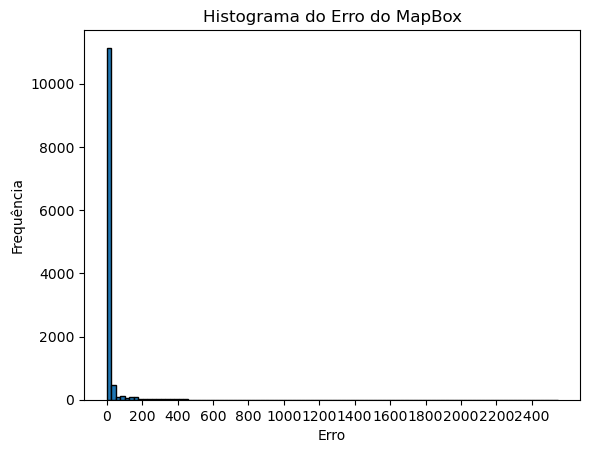
\includegraphics[width=\textwidth]{Figuras/histMapboxSP.png}
    \caption{Mapbox}
    \label{fig:histmapbox}
  \end{subfigure}
  \hfill
  \begin{subfigure}[b]{0.45\textwidth}
    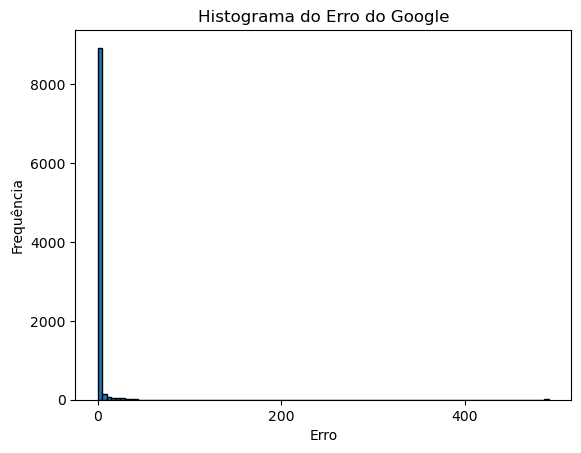
\includegraphics[width=\textwidth]{Figuras/histGoogleSP.png}
    \caption{Google}
    \label{fig:histgoogle}
  \end{subfigure}

  \begin{subfigure}[b]{0.45\textwidth}
    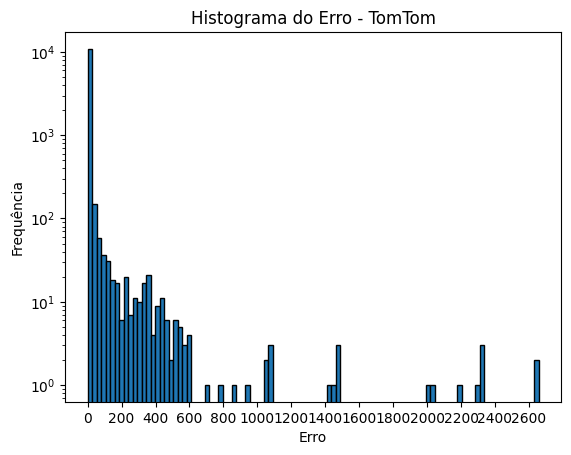
\includegraphics[width=\textwidth]{Figuras/histTomtomSP.png}
    \caption{TomTom}
    \label{fig:histtomtom}
  \end{subfigure}
  \hfill
  \begin{subfigure}[b]{0.45\textwidth}
    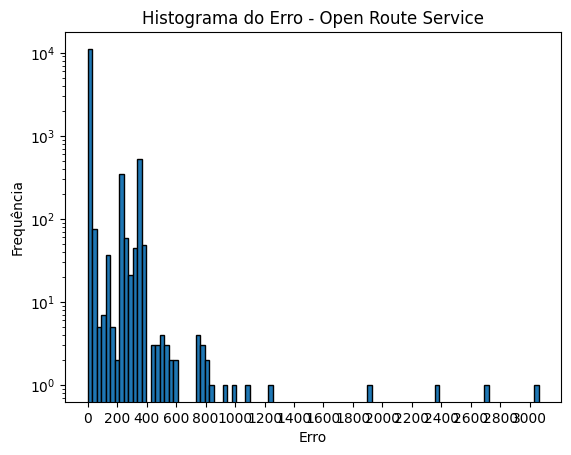
\includegraphics[width=\textwidth]{Figuras/histOrsSP.png}
    \caption{ORS}
    \label{fig:histors}
  \end{subfigure}
  
  \caption{Histogramas do erro das 4 APIs para o todos os dados de São Paulo}
  \label{fig:hist-global-sp}
\end{figure}


\begin{figure}[ht]
  \centering
  \begin{subfigure}[b]{0.45\textwidth}
    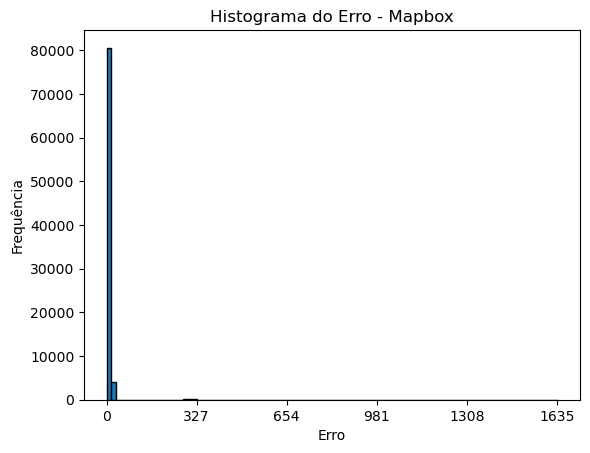
\includegraphics[width=\textwidth]{Figuras/histMapboxBH.png}
    \caption{Mapbox}
    \label{fig:histmapboxb}
  \end{subfigure}
  \hfill
  \begin{subfigure}[b]{0.45\textwidth}
    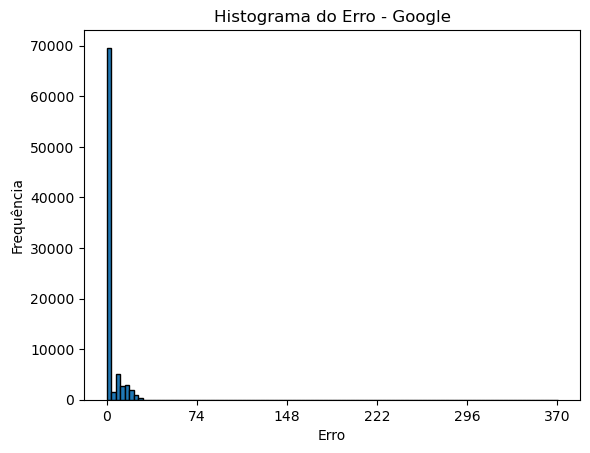
\includegraphics[width=\textwidth]{Figuras/histGoogleBH.png}
    \caption{Google}
    \label{fig:histgoogleB}
  \end{subfigure}

  \begin{subfigure}[b]{0.45\textwidth}
    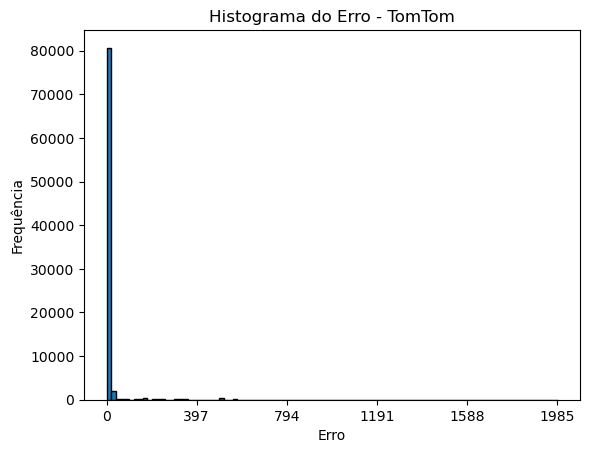
\includegraphics[width=\textwidth]{Figuras/histTomtomBH.png}
    \caption{TomTom}
    \label{fig:histtomtomB}
  \end{subfigure}
  \hfill
  \begin{subfigure}[b]{0.45\textwidth}
    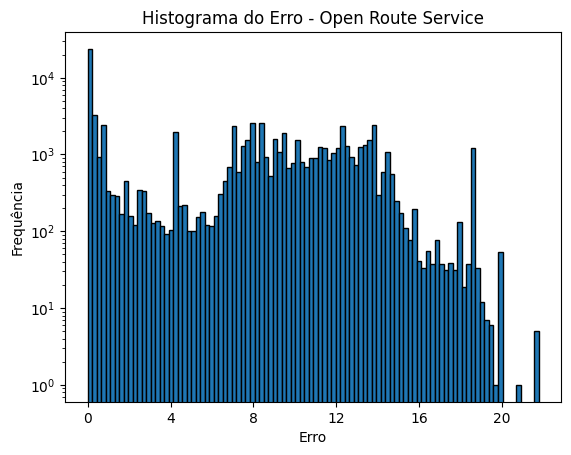
\includegraphics[width=\textwidth]{Figuras/histOrsBH.png}
    \caption{ORS}
    \label{fig:historsB}
  \end{subfigure}
  
  \caption{Histogramas do erro das 4 APIs para o todos os dados de Belo Horizonte}
  \label{fig:hist-global-bh}
\end{figure}


Portanto, decidimos cortar os dados, limitando o erro a 300 metros. Repetimos o processo, gerando um único histograma que representa a distribuição de erro para todas as APIs juntas, para cada uma das bases. 

A figura \ref{fig:histLimitadoSP} mostra o histograma resultante para os dados de São Paulo e a figura \ref{fig:histLimitadoBH} mostra o histograma para os dados de Belo Horizonte. 

Em relação aos dados de São Paulo as APIs tiveram resultados similares nessa faixa de valores do erro. Porém as APIs Google Maps e TomTom se destacaram ao conter uma curva mais estreira, ou seja, os valores para essa API estão mais concentrados em erro menor que 50 metros. 

Para os dados de Belo Horizonte, a API Mapbox teve melhores resultado com uma curva bem estreita. Seguida pela Google Maps, que apesar de ter uma curva bem estreita também, apresenta uma diferença significativa para a Mapbox. As outras APIs apresentam curvas mais largas e algo notável é a curva da mapbox que está muito distribuída, tendo um aspecto parecido com uma reta em valores de erro superiores a 50 metros. Isso mostra que a ORS apresenta erro similar na maior parte da faixa, o que indica que ela não apresenta bons resultados nem quando há um corte nos dados.

\begin{figure}[h]
  \centering
  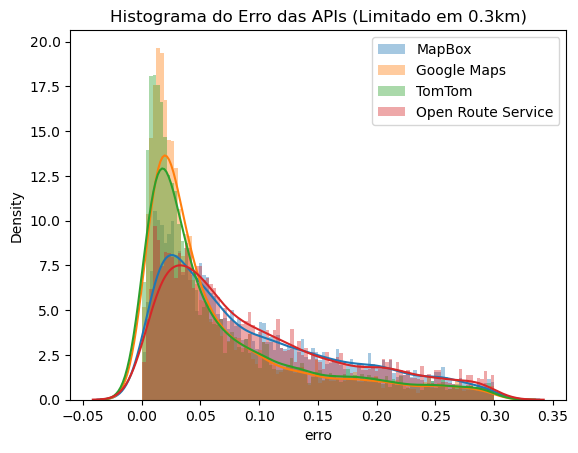
\includegraphics[width=0.7\textwidth]{Figuras/histLimitadoSP.png}
  \caption{Histograma comparativo de erro das APIs limitado em 300 metros para os dados de São Paulo}
  \label{fig:histLimitadoSP}
\end{figure}

\begin{figure}[h]
  \centering
  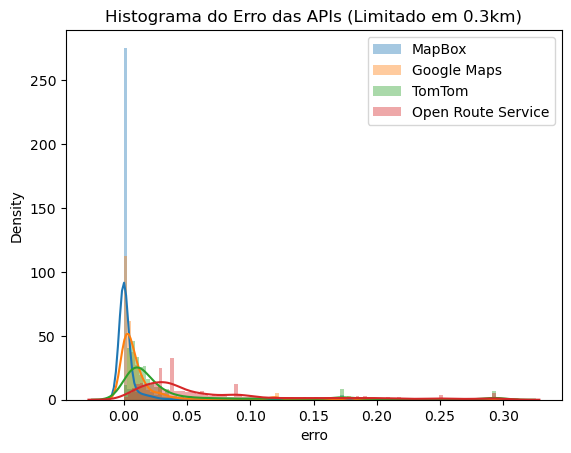
\includegraphics[width=0.7\textwidth]{Figuras/histLimitadoBH.png}
  \caption{Histograma comparativo de erro das APIs limitado em 300 metros para os dados de Belo Horizonte}
  \label{fig:histLimitadoBH}
\end{figure}

Em geral, embora os histogramas sejam uma ferramenta poderosa para analisar a distribuição de erros, neste caso, eles não se mostraram tão eficazes devido às limitações decorrentes da presença de valores excessivamente altos.

\section{Distribuição Espacial do Erro}

Além disso, realizamos uma análise adicional com o objetivo de verificar o comportamento do erro no espaço. Utilizamos gráficos de classificação hexagonal, empregando a função hexbin da biblioteca matplotlib, que desempenha um papel integral na construção do gráfico. Essa função automatiza o processo, dividindo o espaço em hexágonos de tamanhos uniformes e distribuídos de maneira equitativa. Em seguida, a função hexbin seleciona os pontos de dados contidos em cada hexágono e aplica uma função específica, que é definida como parâmetro da função hexbin. Essa função determina os cálculos realizados com base nos pontos, gerando um valor único. Esse valor é então atribuído ao hexágono correspondente no gráfico, e as cores são mapeadas de acordo com uma escala predefinida.

Para gerar a representação do gráfico introduzimos o conceito de "falha". Quando o erro em um ponto específico é igual ou inferior a 150 metros, atribuímos o valor 0 à falha; caso contrário, designamos o valor 1. A função escolhida para calcular o valor de cada hexágono é a média da falha dos pontos, resultando em uma representação em porcentagem decimal da falha naquela região. Assim, quanto mais escura a cor do gráfico, maior é a falha observada. Para melhor vizualização, também adicionamos o limite da cidade como contorno do gráfico. As figuras \ref{fig:falhas-global-bh} e \ref{fig:falhas-global-sp} apresentam os gráficos de falhas de cada uma das APIs para os dados de Belo Horizonte e São Paulo respectivamente. 

Para os dados de Belo Horizonte é possível notar que a API com gráfico mais claro, ou seja, menos falhas, é a Mapbox, seguido pela Google. Resultado que vai de encontro com os obtidos nas tabela de métricas \ref{tab:tabelaDeMetricasBH}. Outra informação relevante que é possível observar é que em todas as APIs existe uma concentração maior de falhas próximo aos limites da cidade, como esperado. Outro ponto importante é o gráfico da ORS. A maior parte do gráfico para essa API apresenta cores bem escuras, indicando muitas falhas em toda região da cidade para essa API. Mais especificamente nas regiões superior e inferior do gráfico o valor chega próximo do limite máximo, o que indica que naquela região houve aproximadamente 100\% de falha. Esse resultado, apesar de ruim, está de acordo com os análises sobre a ORS feitas anteriormente. 

\begin{figure}[ht]
  \centering
  \begin{subfigure}[b]{0.45\textwidth}
    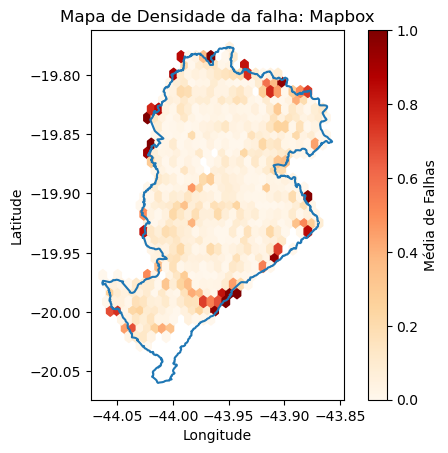
\includegraphics[width=\textwidth]{Figuras/falhasMapboxBH.png}
    \caption{Mapbox}
    \label{fig:falhasmapboxB}
  \end{subfigure}
  \hfill
  \begin{subfigure}[b]{0.45\textwidth}
    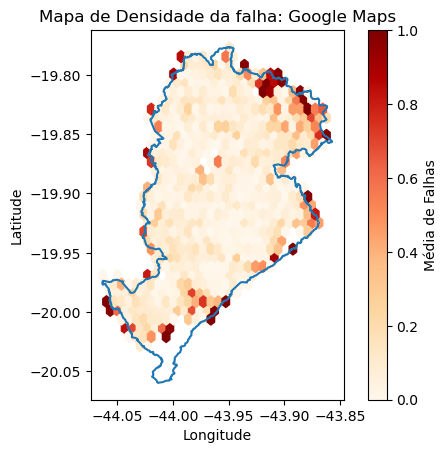
\includegraphics[width=\textwidth]{Figuras/falhasGoogleBH.png}
    \caption{Google}
    \label{fig:falhasgoogleB}
  \end{subfigure}

  \begin{subfigure}[b]{0.45\textwidth}
    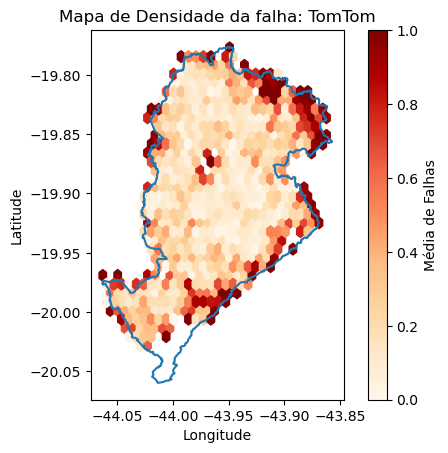
\includegraphics[width=\textwidth]{Figuras/falhasTomtomBH.png}
    \caption{TomTom}
    \label{fig:falhastomtomB}
  \end{subfigure}
  \hfill
  \begin{subfigure}[b]{0.45\textwidth}
    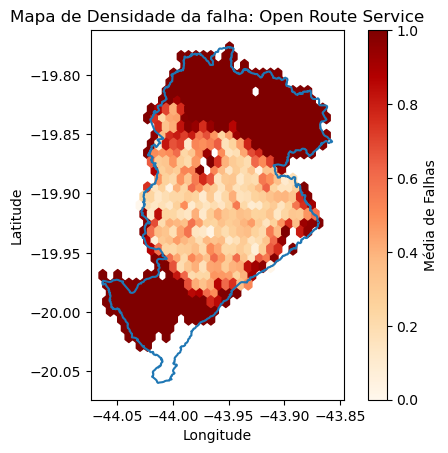
\includegraphics[width=\textwidth]{Figuras/falhasORSBH.png}
    \caption{ORS}
    \label{fig:falhasorsB}
  \end{subfigure}
  
  \caption{Gráficos de falhas de cada API para os dados de Belo Horizonte}
  \label{fig:falhas-global-bh}
\end{figure}

Nos gráficos de São Paulo também foi adicionado o contorno da cidade. No entanto, os dados são referentes a região metropolitana, incluindo outras cidades da região. Para essa base é possível notar que as APIs Google Maps e TomTom tem melhores resultados, o que confirma os resultados obtidos na tabela \ref{tab:tabelaDeMetricasSP}. Outro resultado notável é que nos outros municípios o resultado piora em todas as APIs, atingindo valores de falha muito próximo de 1. Por fim, as APIs que foram piores foram Mapbox e ORS. A ORS foi claramente pior, repetindo os resultado de Belo Horizontes observados nos gráficos da figura \ref{fig:falhas-global-bh} e nas tabelas \ref{tab:tabelaDeMetricasBH} e \ref{tab:tabelaDeMetricasSP}.

\begin{figure}[ht]
  \centering
  \begin{subfigure}[b]{0.45\textwidth}
    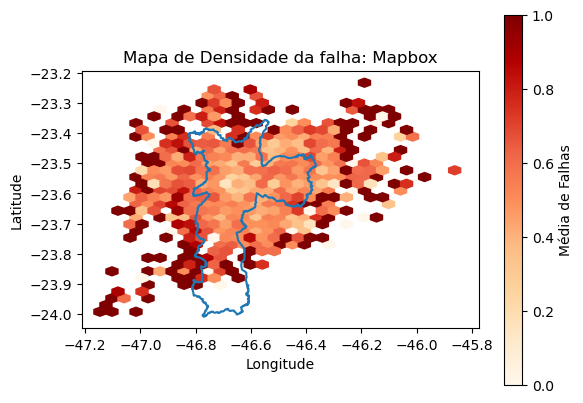
\includegraphics[width=\textwidth]{Figuras/falhasMapboxSP.png}
    \caption{Mapbox}
    \label{fig:falhasmapboxS}
  \end{subfigure}
  \hfill
  \begin{subfigure}[b]{0.45\textwidth}
    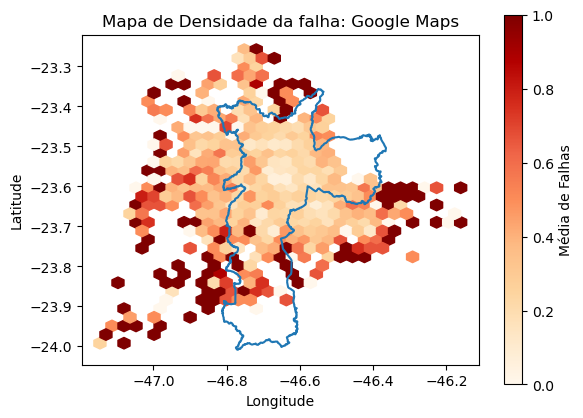
\includegraphics[width=\textwidth]{Figuras/falhasGoogleSP.png}
    \caption{Google}
    \label{fig:falhasgoogleS}
  \end{subfigure}

  \begin{subfigure}[b]{0.45\textwidth}
    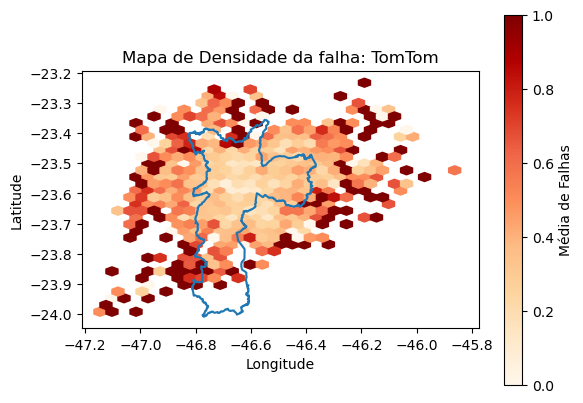
\includegraphics[width=\textwidth]{Figuras/falhasTomtomSP.png}
    \caption{TomTom}
    \label{fig:falhastomtomS}
  \end{subfigure}
  \hfill
  \begin{subfigure}[b]{0.45\textwidth}
    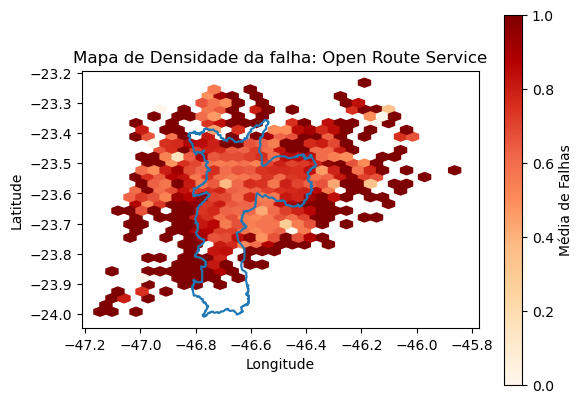
\includegraphics[width=\textwidth]{Figuras/falhasORSSP.png}
    \caption{ORS}
    \label{fig:falhasorsS}
  \end{subfigure}
  
  \caption{Gráficos de falhas de cada API para os dados de Belo São Paulo}
  \label{fig:falhas-global-sp}
\end{figure}

\section{Relações entre erro e discrepância}

Por fim, foi realizada a análise comparativa entre erro e discrepância. As medidas escolhidas para essa análise foram a covariância e a distância para o ponto médio como descrito no capítulo \ref{desenvolvimento}. Foram considerados apenas os endereços em que se tinha informação de todas as APIs. Depois de calcular as métricas para cada um dos pontos foi calculada a correlação de Pearson para cada API e cada base de dados.  

Realizamos então uma análise com um subconjunto de 8574 endereços do banco de dados de São Paulo. A Tabela \ref{tab:correlationSP} exibe esses resultados. A partir da tabela, pode-se observar que para todas as APIs, as correlações com o erro são positivas. Isso indica que à medida que o erro aumenta, as medidas de discrepância também tendem a aumentar. de acordo com a tabela \ref{tab:correlacaoPearson} a medida de covariância para esses dados apresentou uma correlação regular a forte para a maioria das APIs, variando de 0,53 a 0,67, exceto para o Google Maps, que teve uma correlação fraca. Por outro lado, a medida de distância até o ponto médio obteve uma correlação forte a muito forte para a maioria das APIs, com resultados na faixa de 0,88 a 0,94. Em contrapartida, a API do Google mostrou uma correlação regular muito próxima a fraca, mas houve uma melhoria em comparação com a correlação de covariância.

\begin{table}[h]
\centering
\caption{Correlação  de Pearson entre Erro e Medidas de Discrepância para São Paulo}
\label{tab:correlationSP}
\begin{adjustbox}{width=0.7\textwidth}
\begin{tabular}{|c|c|c|}
\hline
API & Covariância & Distância até o Ponto Médio \\
\hline
Mapbox & 0,5387 & 0,8972 \\
TomTom & 0,5398 & 0,8858 \\
Google & 0,2177 & 0,3615 \\
ORS & 0,6649 & 0,9378 \\
\hline
\end{tabular}
\end{adjustbox}
\end{table}

Para o conjunto de dados de Belo Horizonte, conduzimos essa análise com 84.752 endereços, o que representa aproximadamente 99,71\% da amostra utilizada. A Tabela \ref{tab:correlationBH} mostra esses resultados. Em geral, a tabela apresenta valores de correlação mais próximos de 0 do que os encontrados na análise dos dados de São Paulo, indicando que a correlação é mais fraca para este conjunto de dados como um todo. Para o Google e o ORS, a covariância mostrou uma correlação fraca, possivelmente indicando nenhuma relação entre erro e covariância para essas APIs. O Mapbox teve uma correlação regular com a covariância, enquanto o TomTom teve uma correlação forte.

Para a distância até o ponto médio, tivemos correlações fortes a muito fortes para o Mapbox e o TomTom. O Google e o ORS também apresentaram correlações fracas para a distância do ponto médio. Apesar dos resultados de correlação inferiores em comparação com a análise do conjunto de dados de São Paulo, os resultados de Belo Horizonte parecem confirmar que distância até o ponto médio é uma medida melhor em comparação com a covariância para substituir o erro em situações onde o mesmo não pode ser obtido.

\begin{table}[!ht]
\centering
\caption{Correlação de Pearson entre Erro e Medidas de Discrepância para Belo Horizonte}
\label{tab:correlationBH}
\begin{adjustbox}{width=0.7\textwidth}
\begin{tabular}{|c|c|c|}
\hline
API & Covariância & Distância até o Ponto Médio \\
\hline
Mapbox & 0,4669 & 0,7764 \\
TomTom & 0,7269 & 0,9873 \\
Google & 0,0463 & 0,0754 \\
ORS & 0,1552 & 0,2775 \\
\hline
\end{tabular}
\end{adjustbox}
\end{table}


\section{Experimentos de formatação}

\begin{table}[!ht]
\centering
\caption{Taxa de resposta de cada API por experimento de Belo Horizonte}
\label{tab:txRespExpAPIBH}
\begin{adjustbox}{width=0.7\textwidth}
\begin{tabular}{|c|c|c|c|c|}
\hline
Experimento & MapBox & Google & TomTom & ORS\\
\hline
1 & 100,00 & 99,92 & 100,00 & 99,92\\
\hline
1b &  &  &  & \\
\hline
2 & 100,00 & 99,98 & 99,94 & 99,06\\
\hline
2b & 99,94 & 99,84 & 99,98 & 95,30\\
\hline
3 & 100,00 & 99,92 & 100,00 & 99,04\\
\hline
3b & 99,68 & 100,00 & 99,88 & 99,06\\
\hline
4 & 100,00 & 99,90 & 99,98 & 100,00\\
\hline
4b & 99,92 & 99,92 & 99,98 & 95,12\\
\hline
5 & 99,92 & 99,92 & 99,94 & 99,58\\
\hline
5b & 99,76 & 99,88 & 99,92 & 99,98\\
\hline
\end{tabular}
\end{adjustbox}
\end{table}


\begin{table}[!ht]
\centering
\caption{Taxa de acerto de cada API por experimento de Belo Horizonte}
\label{tab:txRespExpAPIBH}
\begin{adjustbox}{width=0.7\textwidth}
\begin{tabular}{|c|c|c|c|c|}
\hline
Experimento & MapBox & Google & TomTom & ORS\\
\hline
1 & 85,06 & 72,72 & 52,80 & 26,46\\
\hline
1b &  &  &  & \\
\hline
2 & 82,46 & 73,30 & 55,66 & 22,28\\
\hline
2b & 79,82 & 78,02 & 53,76 & 5,46\\
\hline
3 & 84,00 & 73,38 & 55,82 & 40,06\\
\hline
3b & 80,56 & 78,30 & 53,92 & 39,08\\
\hline
4 & 84,66 & 73,26 & 55,32 & 1,46\\
\hline
4b & 79,86 & 77,78 & 53,76 & 6,72\\
\hline
5 & 83,80 & 73,32 & 55,78 & 1,48\\
\hline
5b & 81,00 & 72,92 & 53,92 & 24,78\\
\hline
\end{tabular}
\end{adjustbox}
\end{table}

\begin{figure}[ht]
  \centering
  \begin{subfigure}[b]{0.45\textwidth}
    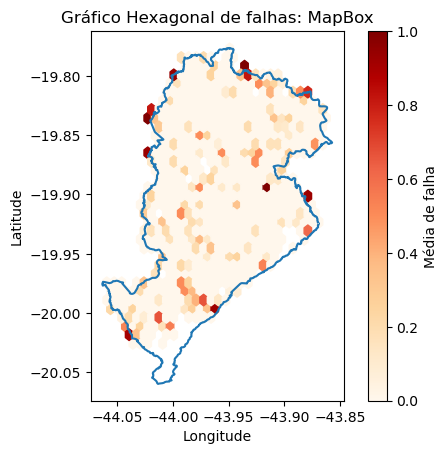
\includegraphics[width=\textwidth]{Figuras/falhasMapboxBHexpG.png}
    \caption{Mapbox: Experimento 1}
    \label{fig:falhasmapboxBexp}
  \end{subfigure}
  \hfill
  \begin{subfigure}[b]{0.45\textwidth}
    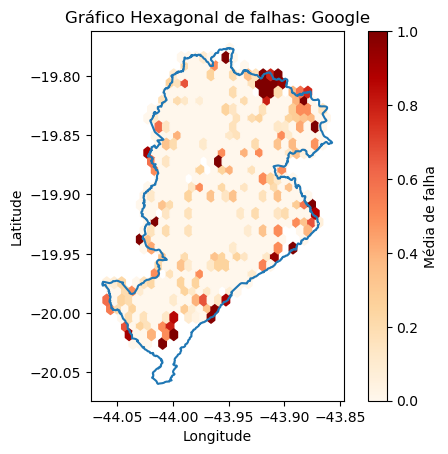
\includegraphics[width=\textwidth]{Figuras/falhasGoogleBHexpG.png}
    \caption{Google: Experimento 3b}
    \label{fig:falhasgoogleBexp}
  \end{subfigure}

  \begin{subfigure}[b]{0.45\textwidth}
    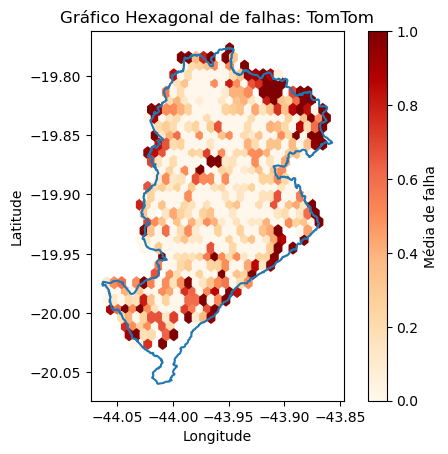
\includegraphics[width=\textwidth]{Figuras/falhasTomtomBHexpG.png}
    \caption{TomTom: Experimento 3}
    \label{fig:falhastomtomBexp}
  \end{subfigure}
  \hfill
  \begin{subfigure}[b]{0.45\textwidth}
    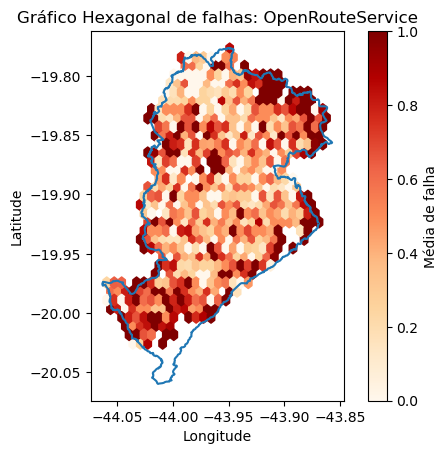
\includegraphics[width=\textwidth]{Figuras/falhasOrsBHexpG.png}
    \caption{ORS: Experimento 3}
    \label{fig:falhasorsBexp}
  \end{subfigure}
  
  \caption{Gráficos de falhas para o melhor desempenho nos experimentos de cada API para os dados de Belo Horizonte}
  \label{fig:falhas-global-bh-exp}
\end{figure}

Box plot completo:

\begin{figure}[h]
    \centering
    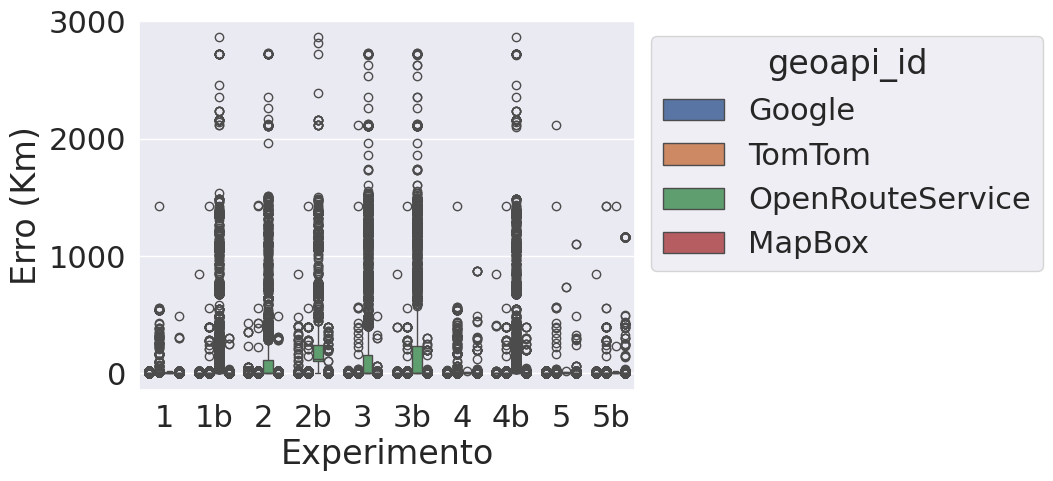
\includegraphics[width=\textwidth]{Figuras/boxplotExperimento.png}
    \caption{Boxplot de Experimentos por Erro, com todas as APIs avaliadas }
    \label{fig:boxplot-completo}
\end{figure}

Boxplot completo sem outliers

\begin{figure}[h]
    \centering
    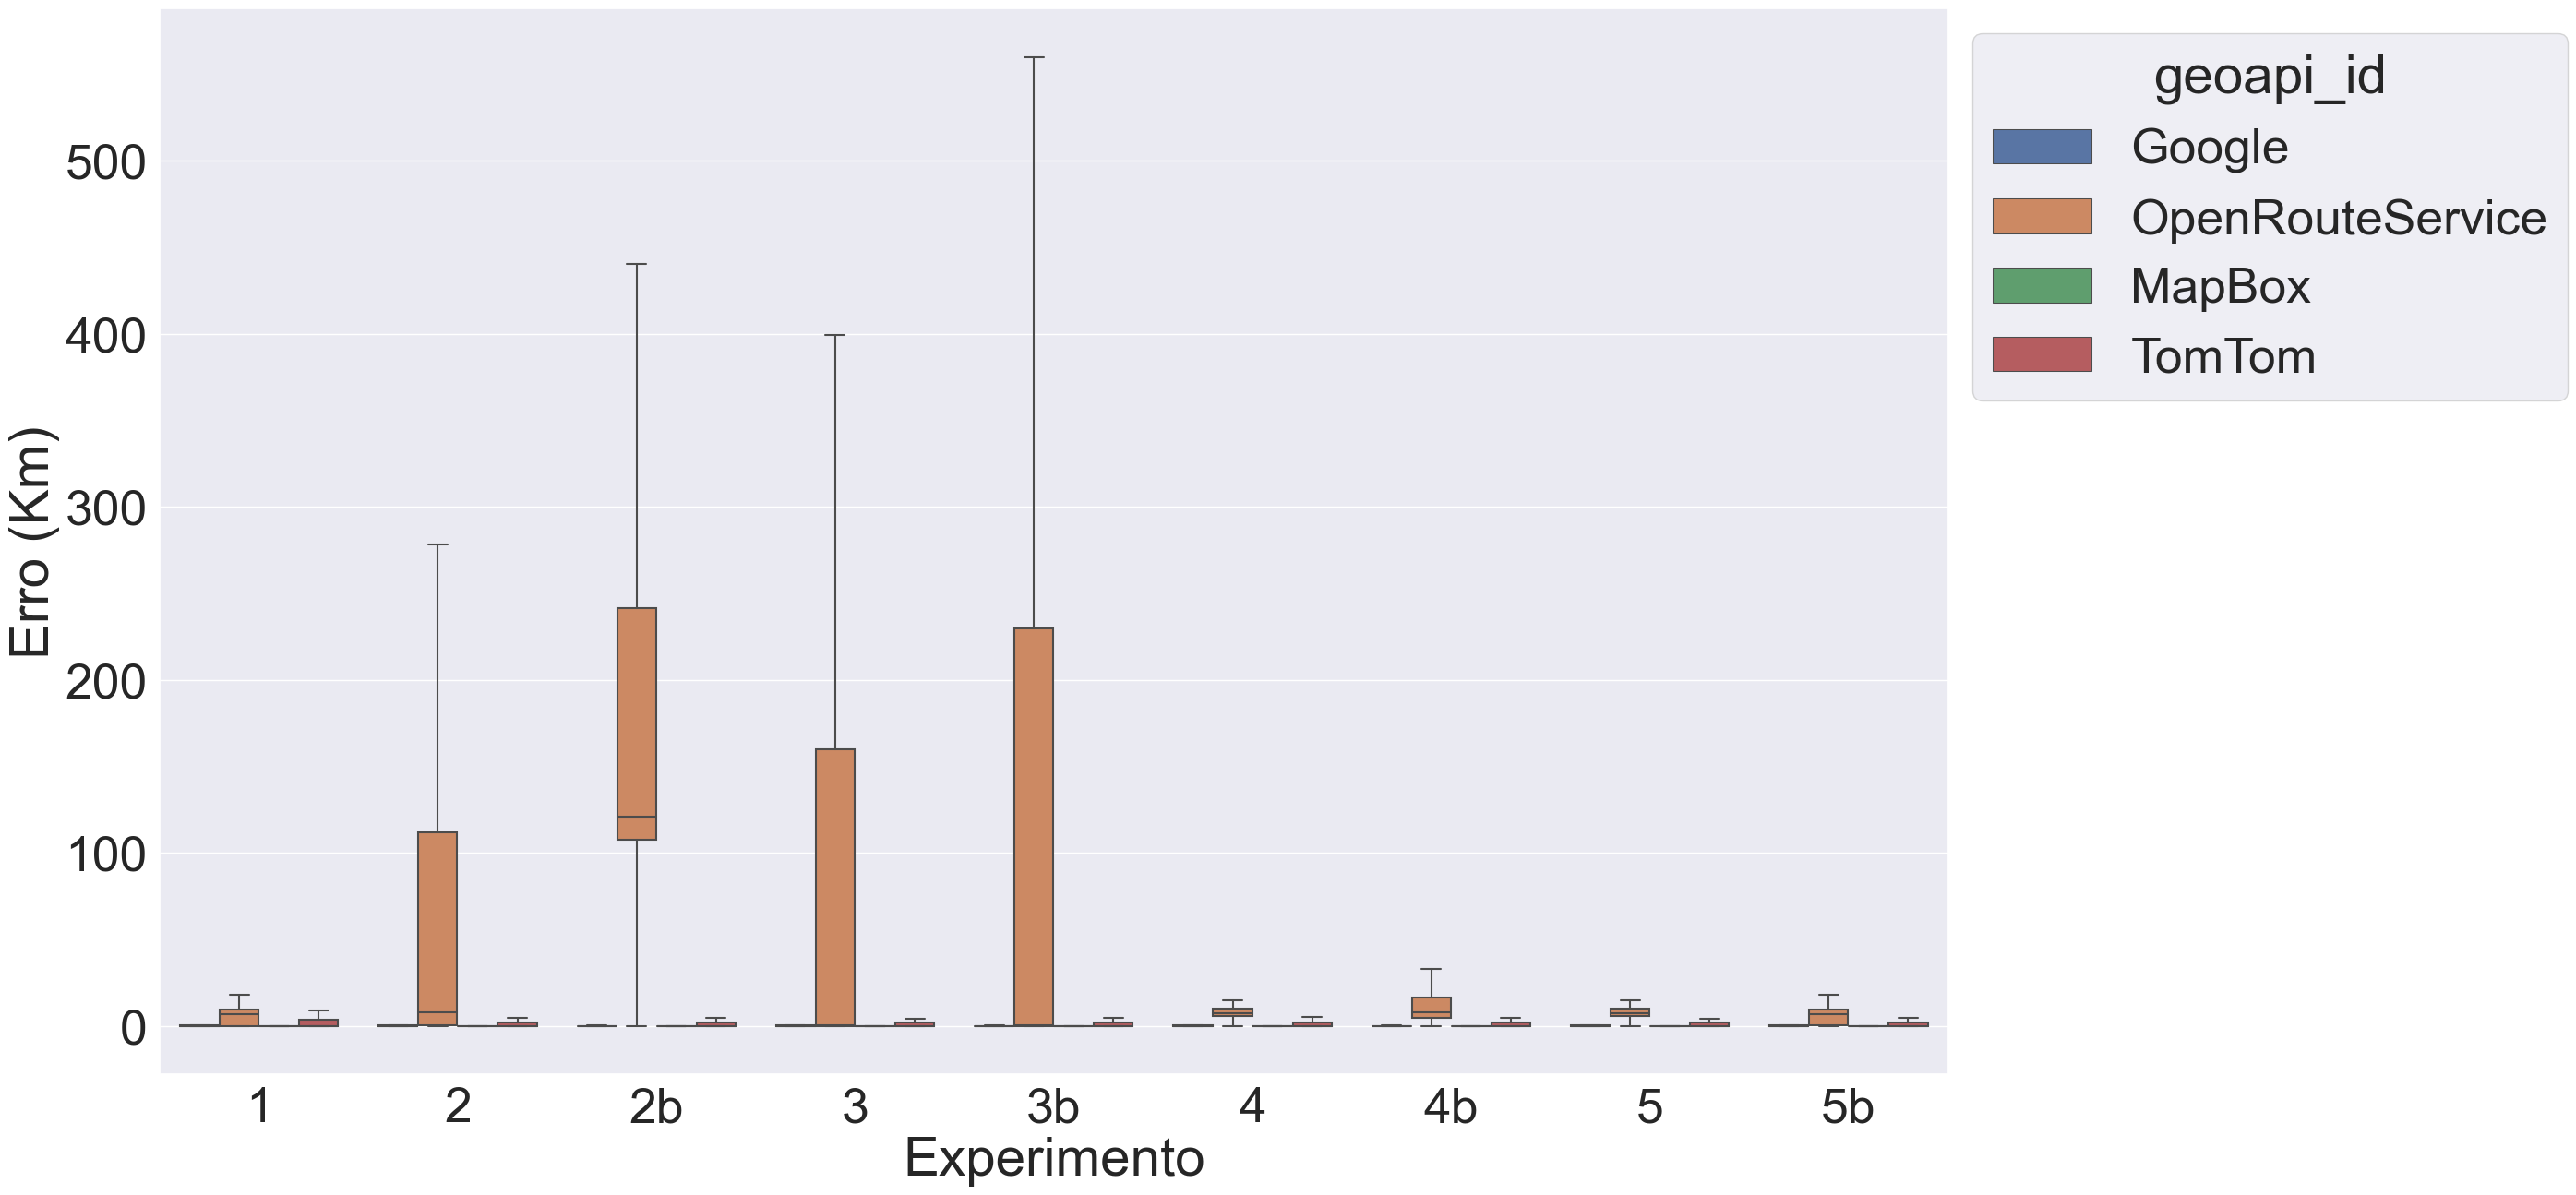
\includegraphics[width=\textwidth]{Figuras/boxplotExperimentoSemOut.png}
    \caption{Boxplot de Experimentos por Erro, com todas as APIs avaliadas e sem Outliers}
    \label{fig:boxplot-semout}
\end{figure}

Boxplot sem ORS:

\begin{figure}[h]
    \centering
    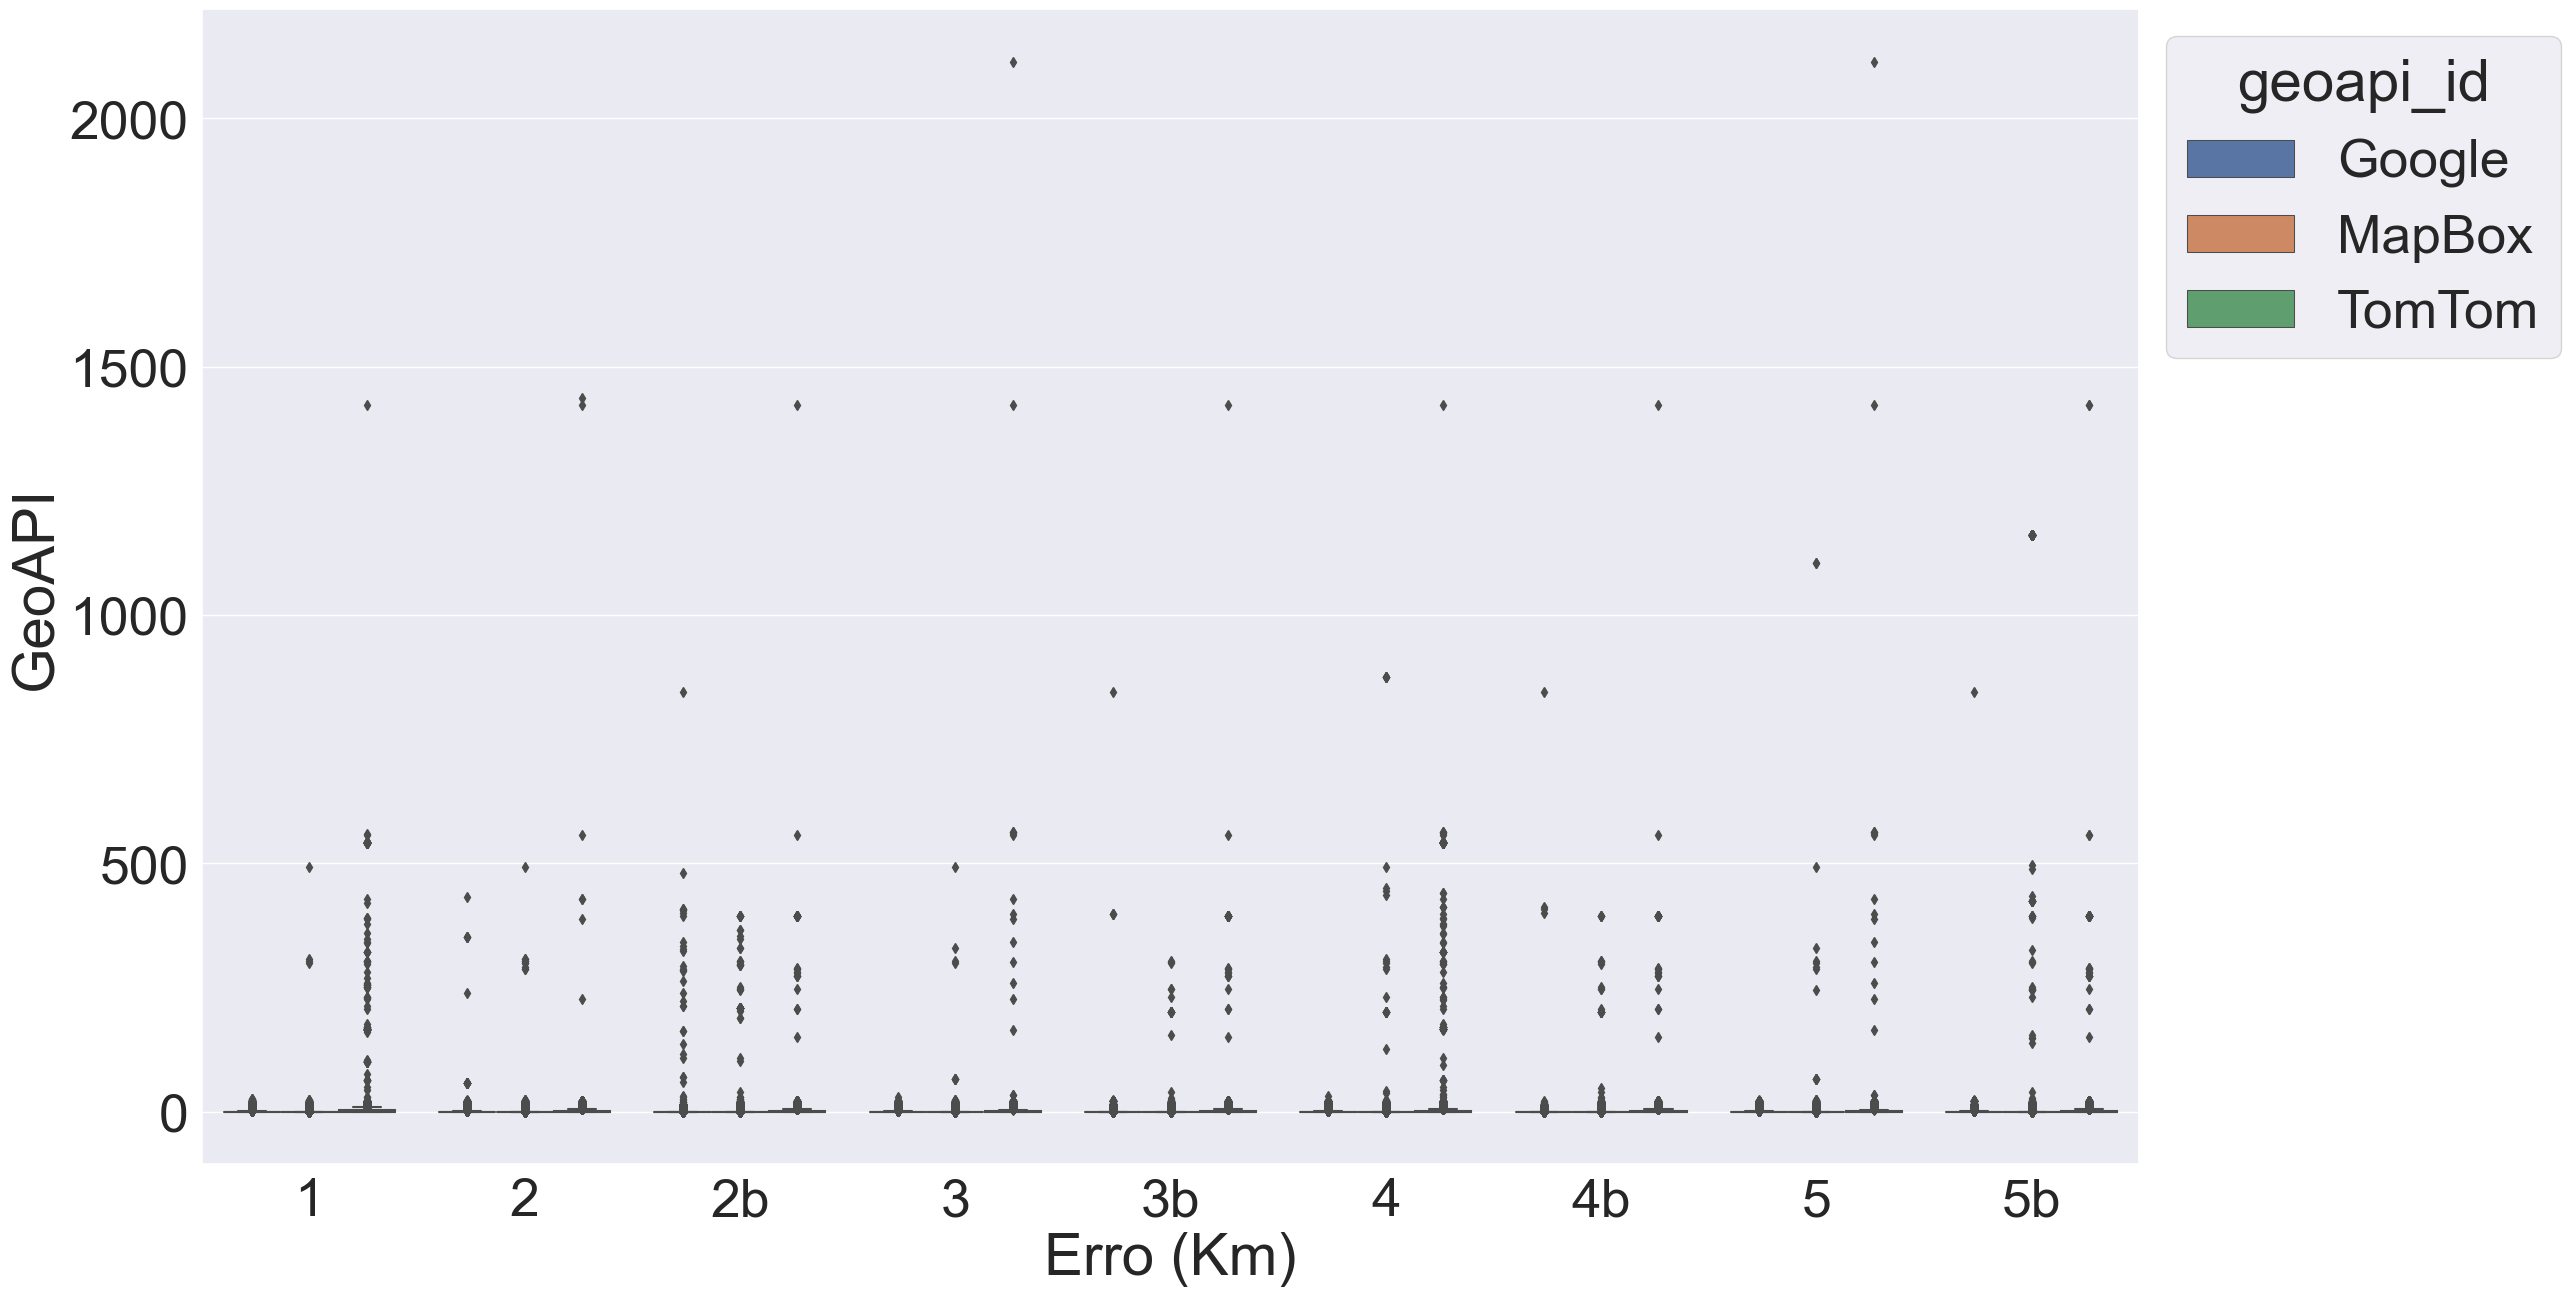
\includegraphics[width=\textwidth]{Figuras/boxplotExperimentoSemORS.png}
    \caption{Boxplot de Experimentos por Erro, com todas as APIs avaliadas exceto ORS}
    \label{fig:boxplot-semors}
\end{figure}

Boxplot sem ORS e sem ouliers:

\begin{figure}[h]
    \centering
    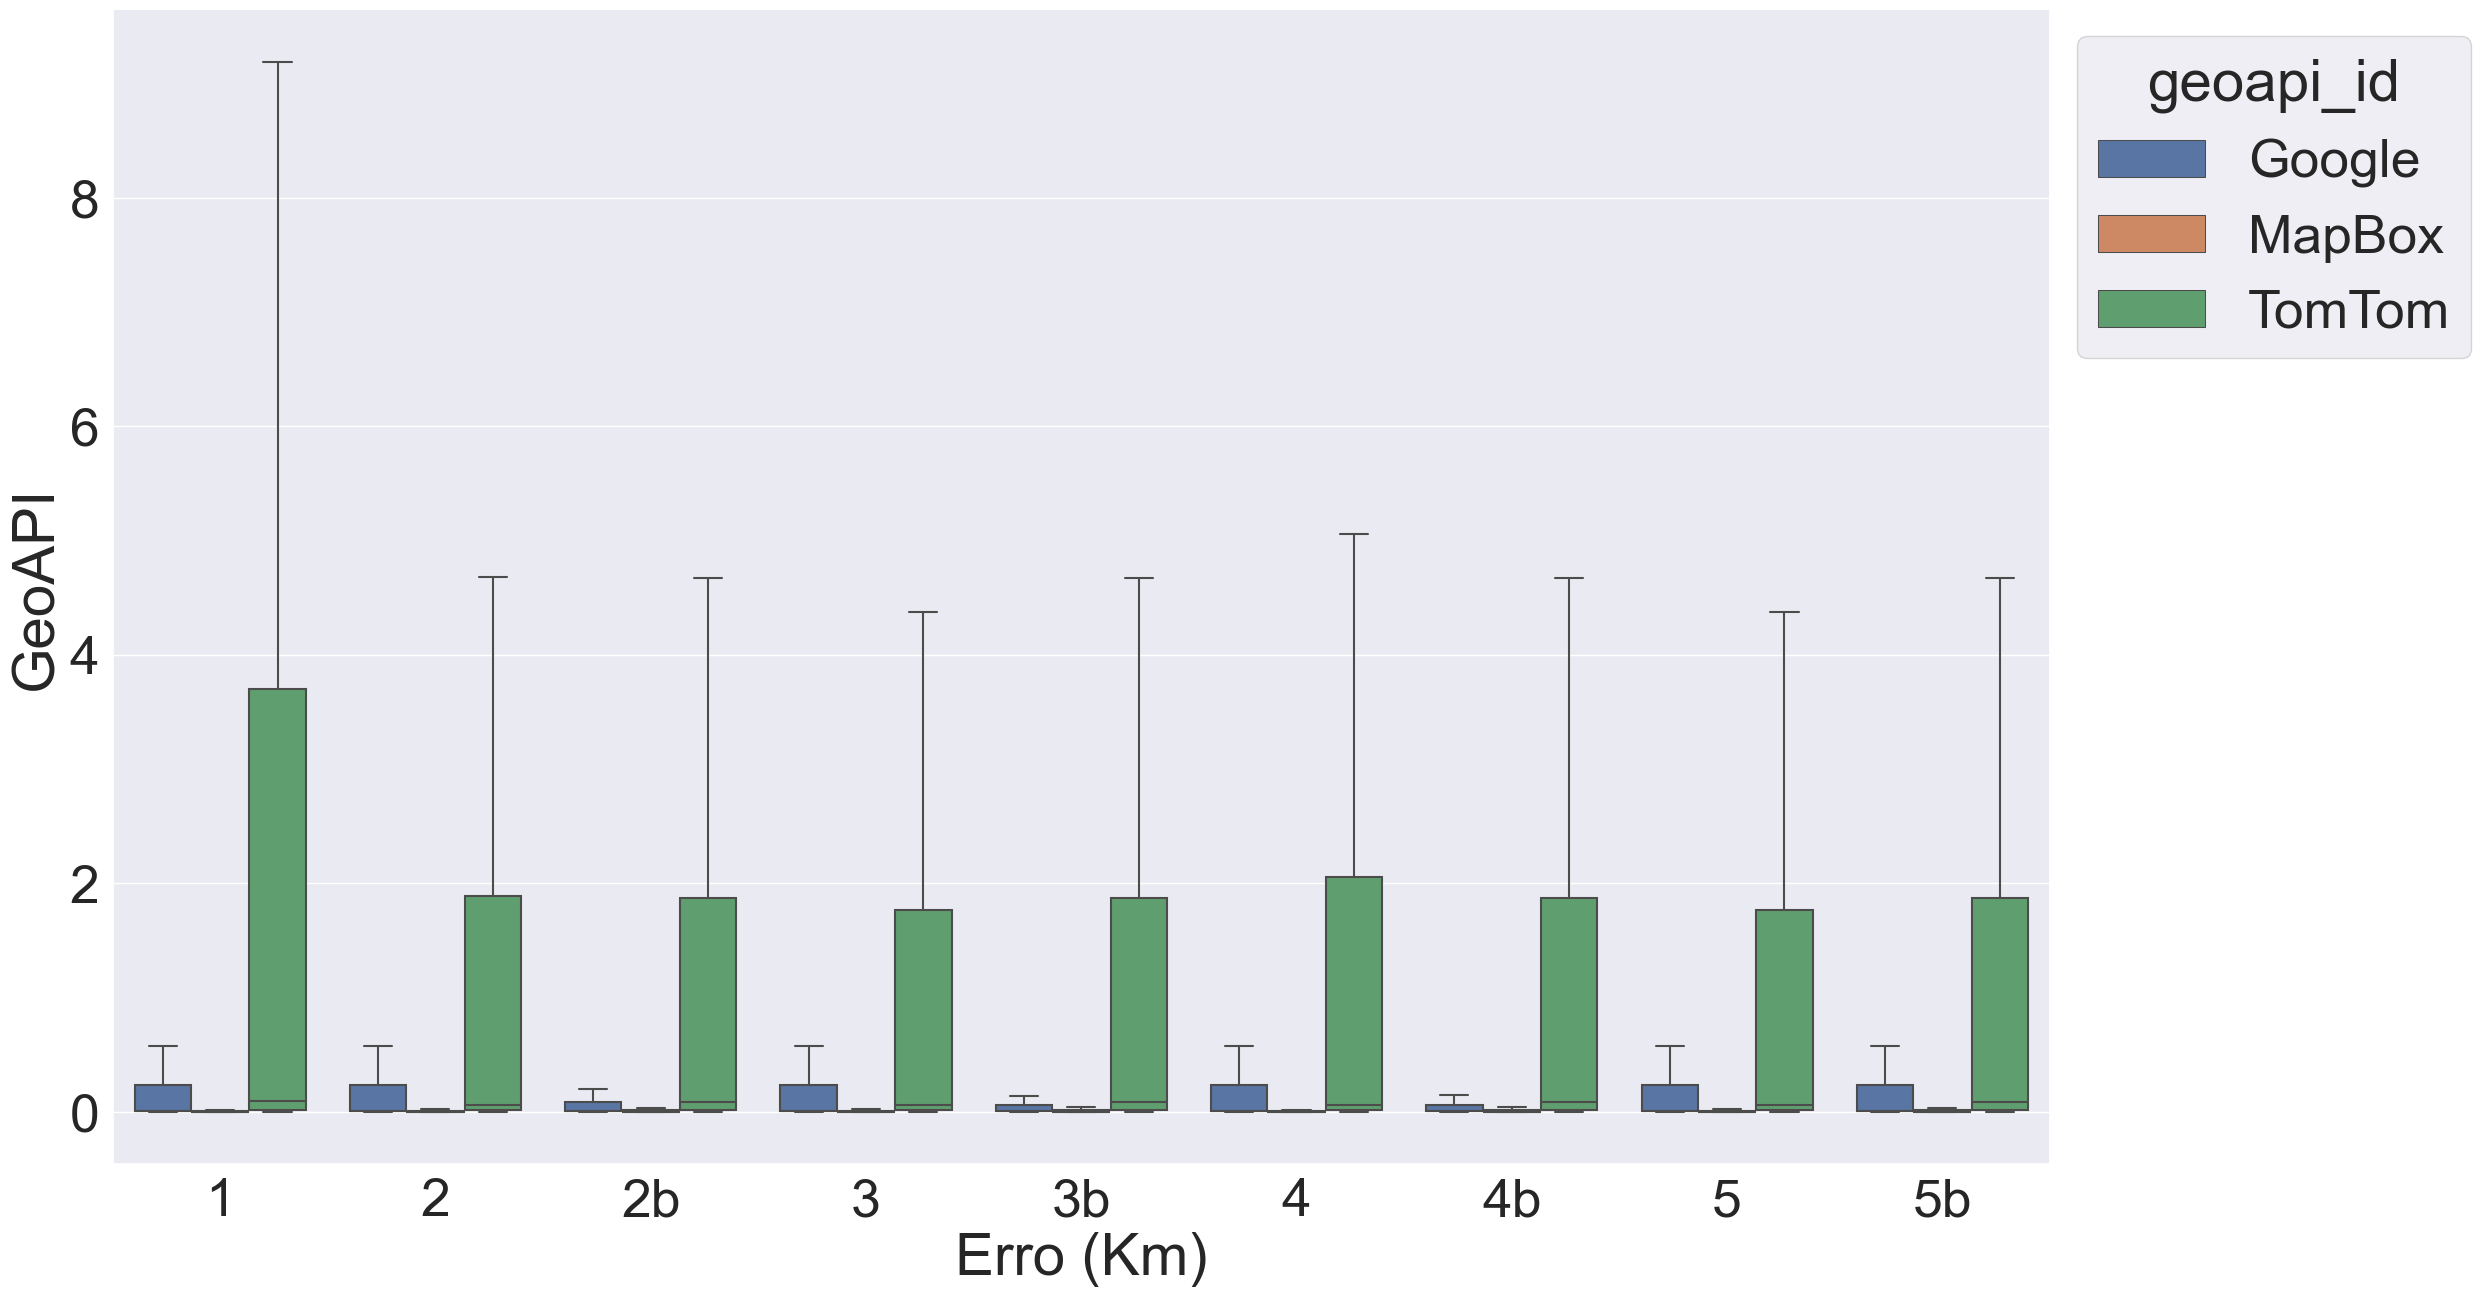
\includegraphics[width=\textwidth]{Figuras/boxplotExperimentoSemOutSemORS.png}
    \caption{Boxplot de Experimentos por Erro, com todas as APIs avaliadas exceto ORS e sem Outliers}
    \label{fig:boxplot-semors-semout}
\end{figure}

Boxplots de API por erro sem completos:

\begin{figure}[ht]
  \centering
  \begin{subfigure}[b]{0.45\textwidth}
    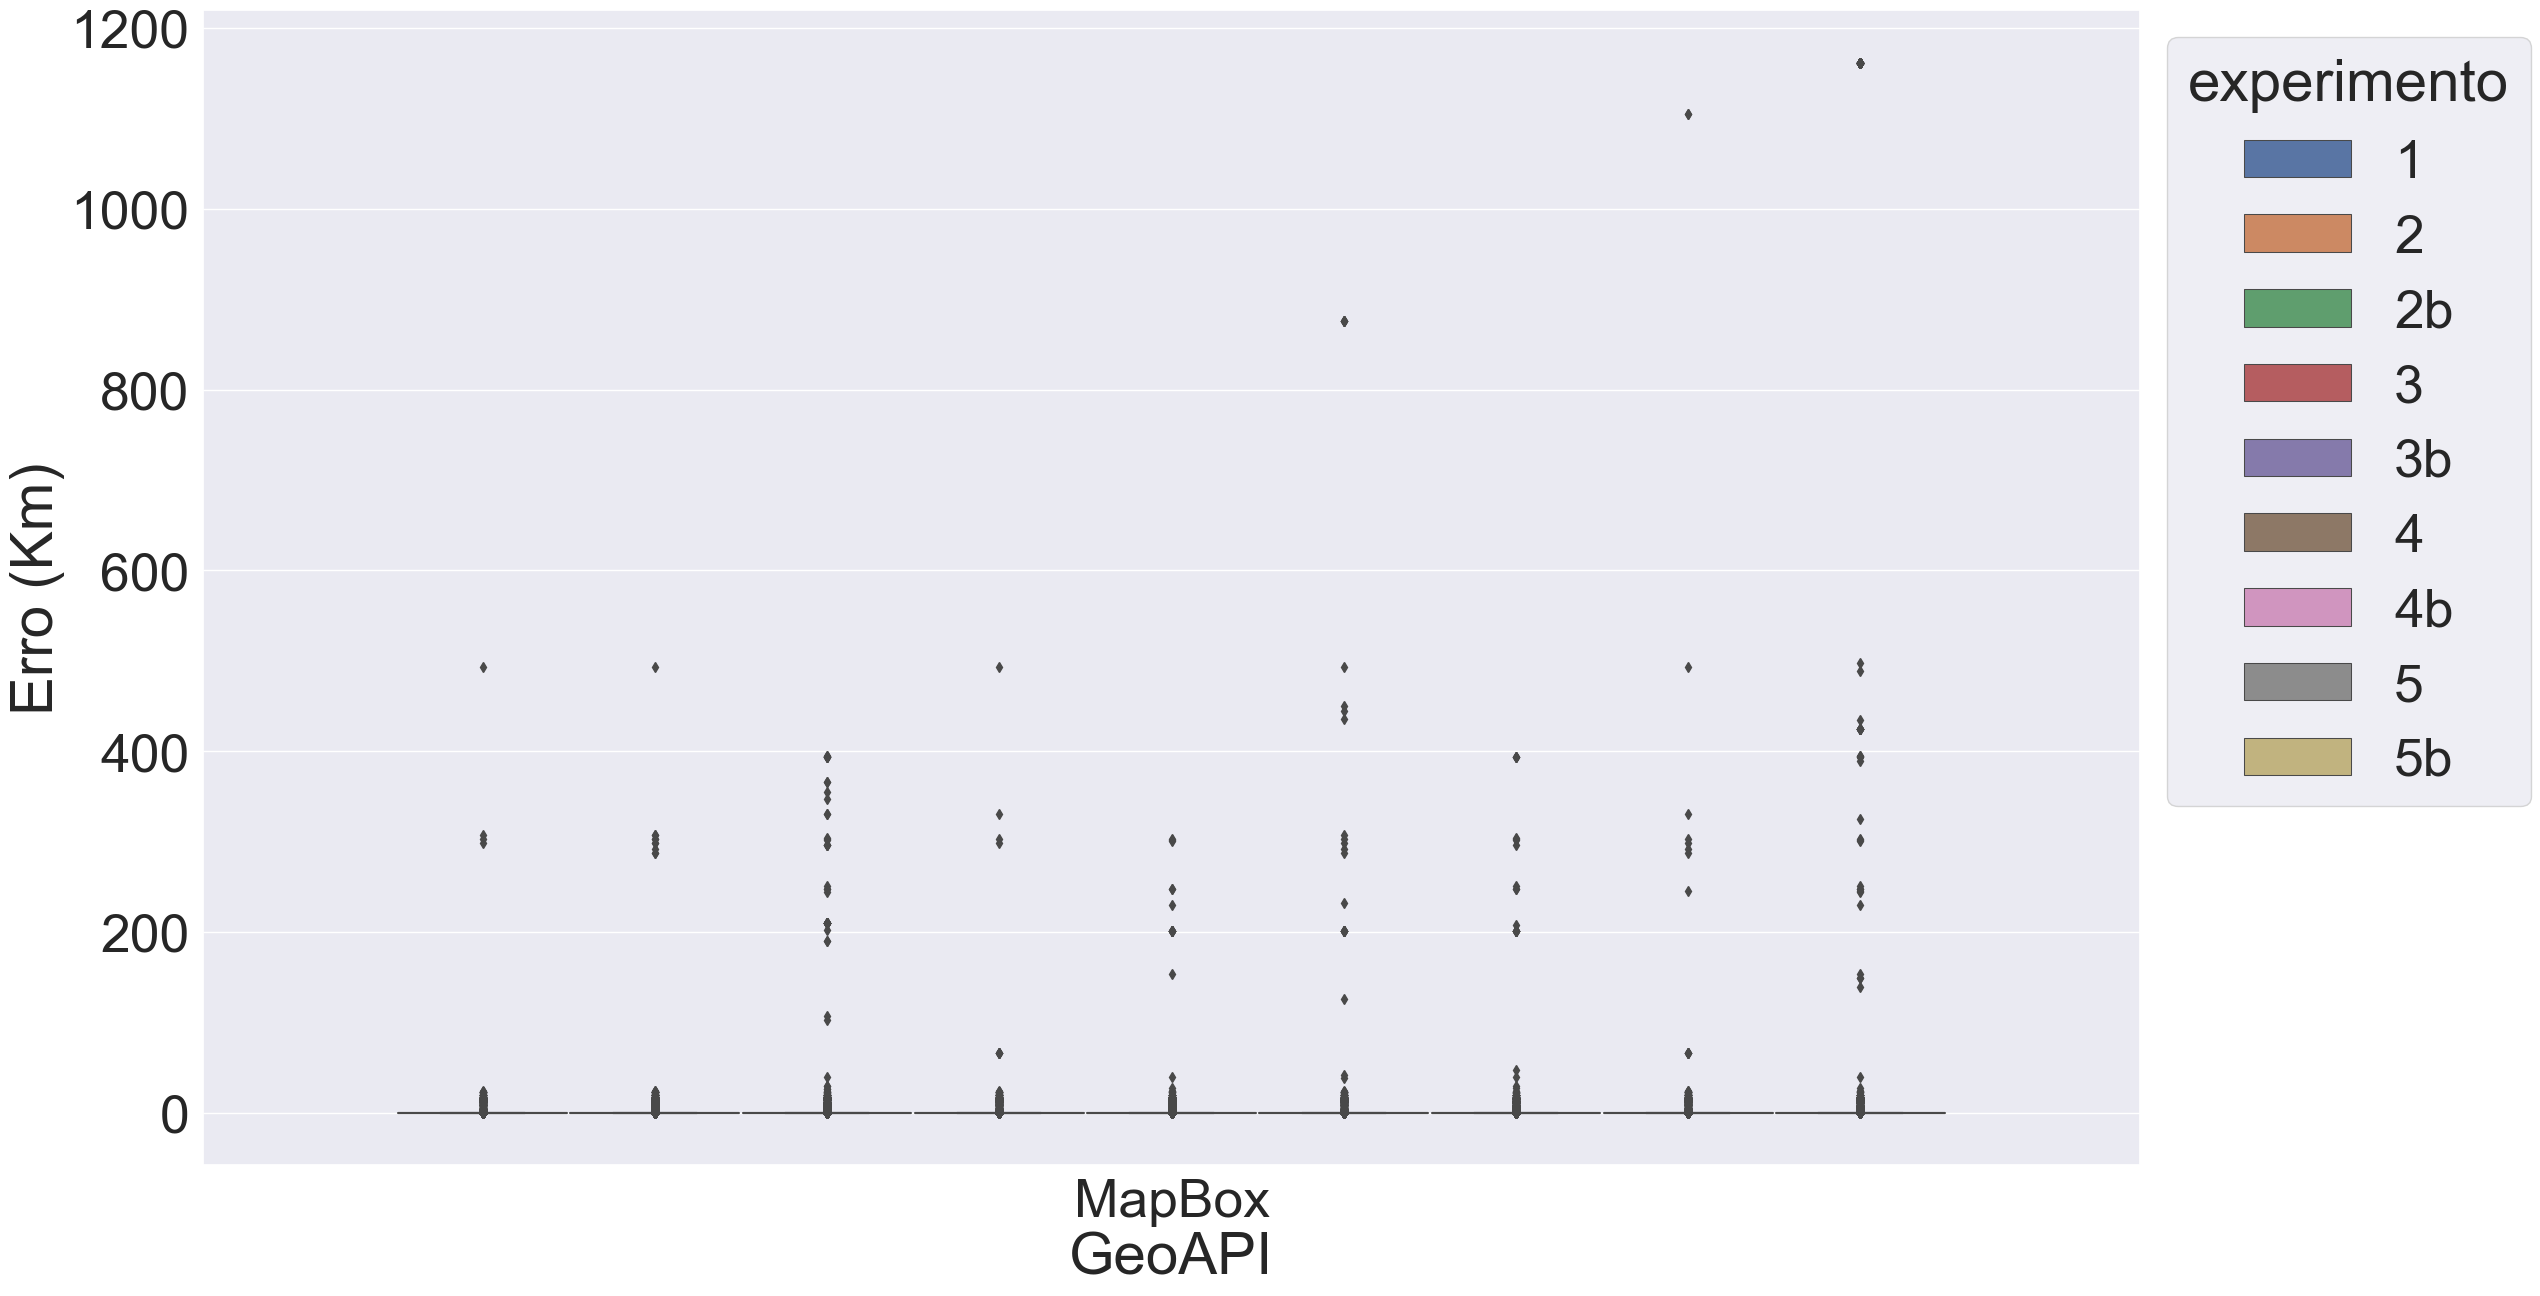
\includegraphics[width=\textwidth]{Figuras/boxplotApiMapbox.png}
    \caption{Mapbox}
    \label{fig:boxplot-api-mapbox}
  \end{subfigure}
  \hfill
  \begin{subfigure}[b]{0.45\textwidth}
    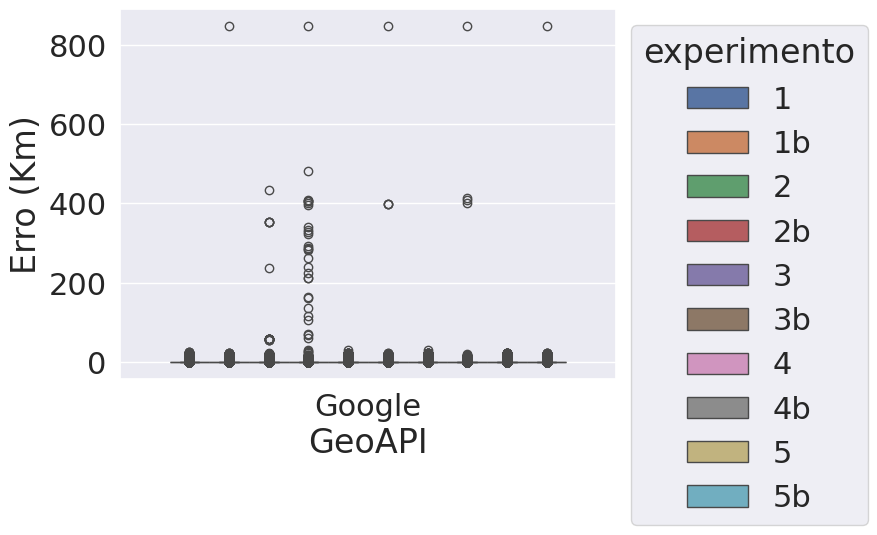
\includegraphics[width=\textwidth]{Figuras/boxplotApiGoogle.png}
    \caption{Google}
    \label{fig:boxplot-api-google}
  \end{subfigure}

  \begin{subfigure}[b]{0.45\textwidth}
    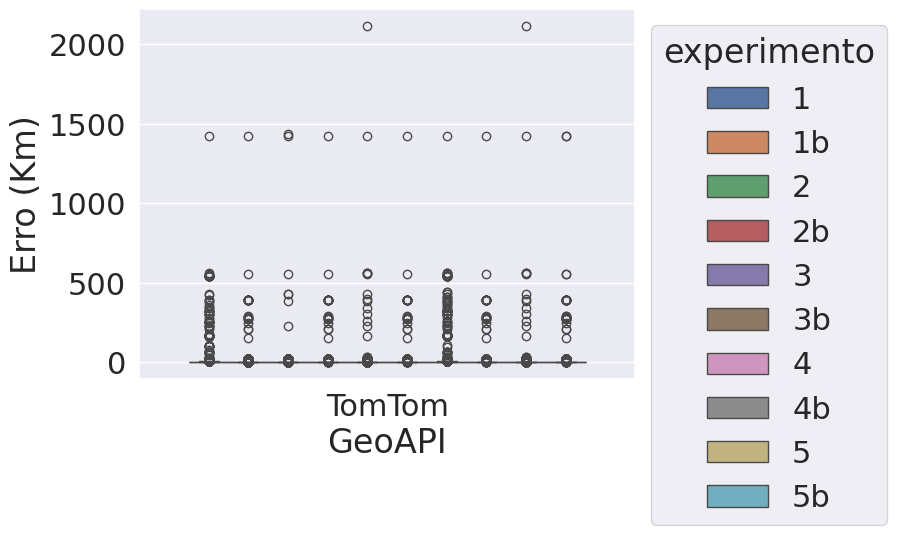
\includegraphics[width=\textwidth]{Figuras/boxplotApiTomtom.png}
    \caption{TomTom}
    \label{fig:boxplot-api-tomtom}
  \end{subfigure}
  \hfill
  \begin{subfigure}[b]{0.45\textwidth}
    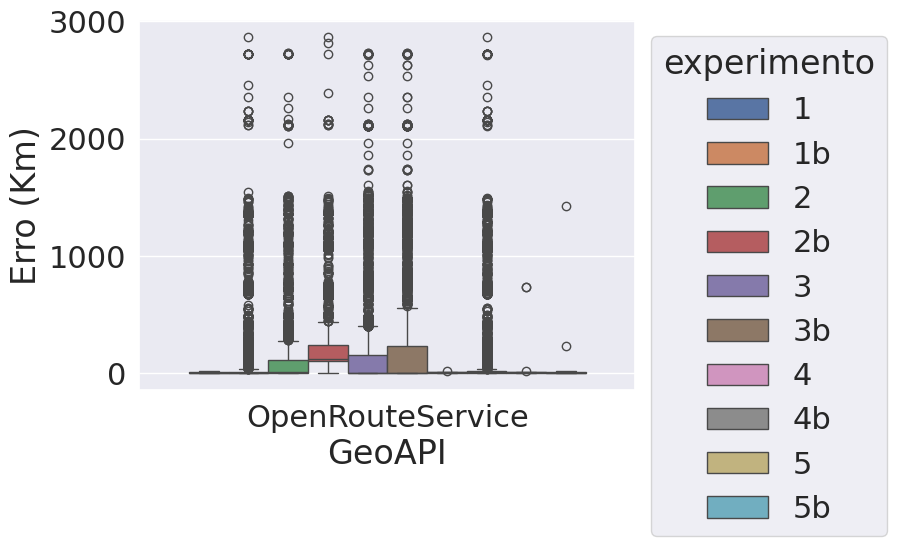
\includegraphics[width=\textwidth]{Figuras/boxplotApiOrs.png}
    \caption{ORS}
    \label{fig:boxplot-api-ors}
  \end{subfigure}
  
  \caption{Boxplots de Erro por API para cada uma das APIs avalidas}
  \label{fig:boxplot-api-global-bh}
\end{figure}

Boxplot Mapbox sem ouliers:

\begin{figure}[h]
    \centering
    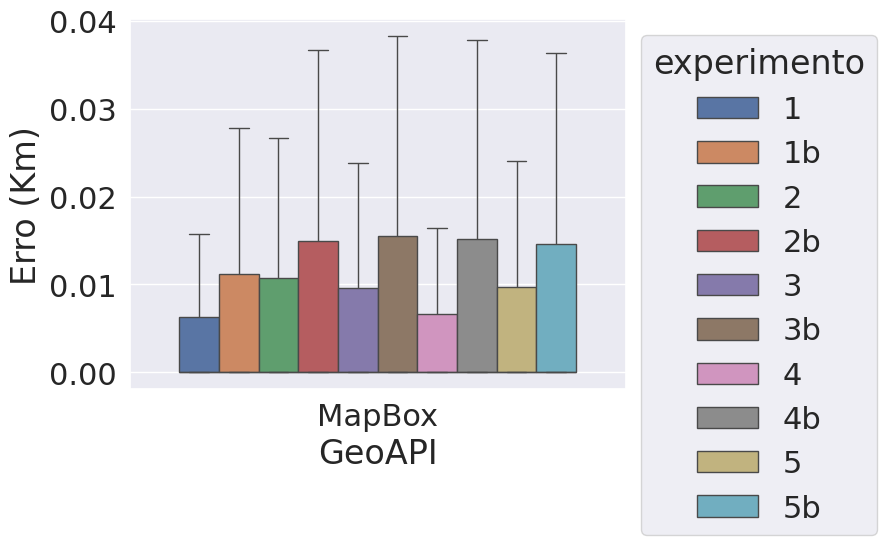
\includegraphics[width=\textwidth]{Figuras/boxplotApiMapboxSemOut.png}
    \caption{Boxplot de Erro por API com todos os experimentos avaliados sem Outliers: Mapbox}
    \label{fig:boxplot-api-mapbox-semout}
\end{figure}

Boxplot Google sem ouliers:

\begin{figure}[h]
    \centering
    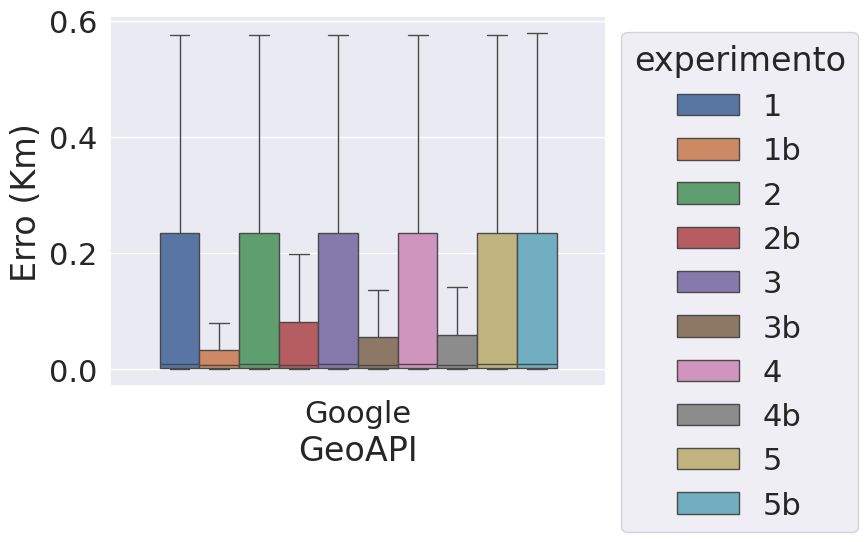
\includegraphics[width=\textwidth]{Figuras/boxplotApiGoogleSemOut.png}
    \caption{Boxplot de Erro por API com todos os experimentos avaliados sem Outliers: Google}
    \label{fig:boxplot-api-google-semout}
\end{figure}

Boxplot TomTom sem ouliers:

\begin{figure}[h]
    \centering
    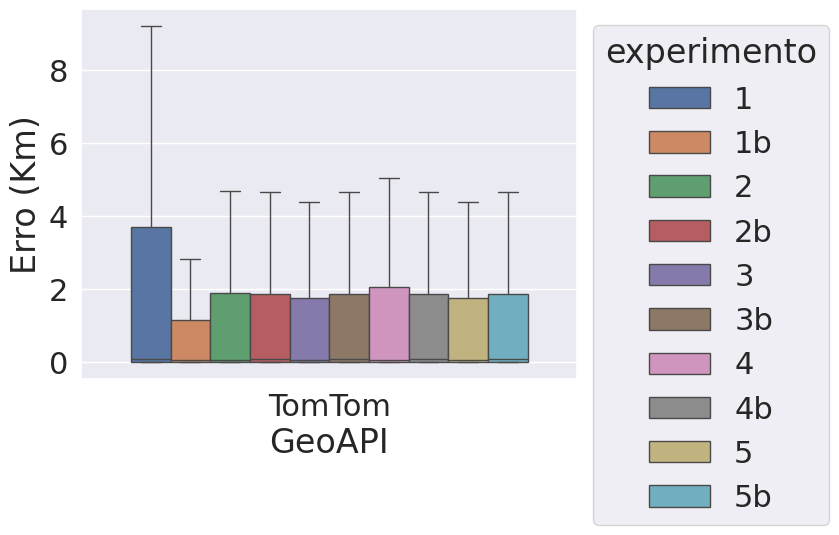
\includegraphics[width=\textwidth]{Figuras/boxplotApiTomtomSemOut.png}
    \caption{Boxplot de Erro por API com todos os experimentos avaliados sem Outliers: TomTom}
    \label{fig:boxplot-api-tomtom-semout}
\end{figure}

Boxplot ORS sem ouliers:

\begin{figure}[h]
    \centering
    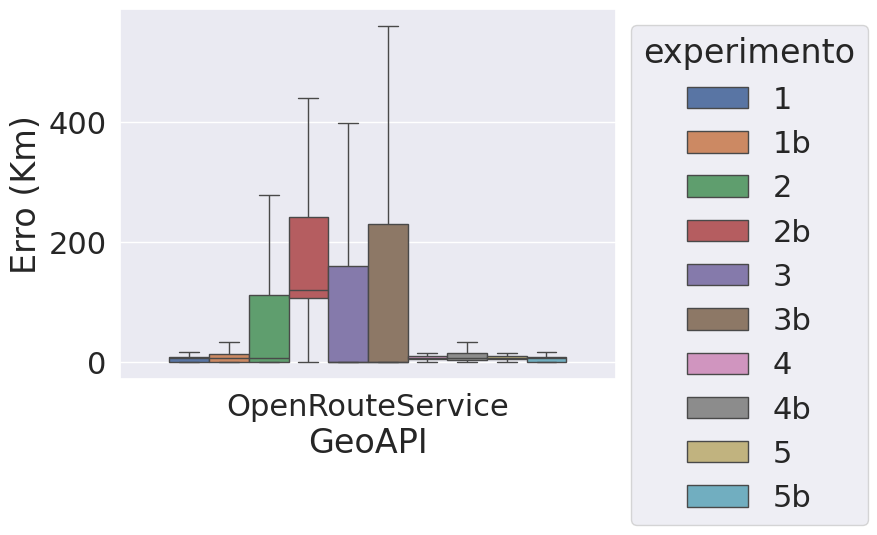
\includegraphics[width=\textwidth]{Figuras/boxplotApiOrsSemOut.png}
    \caption{Boxplot de Erro por API com todos os experimentos avaliados sem Outliers: ORS}
    \label{fig:boxplot-api-ors-semout}
\end{figure}